\documentclass[leqno]{article}
% Shared QBT/Soln pack preamble for resources.danieljsmith.org.
\usepackage{graphicx}
\usepackage{dsfont}
\usepackage{mathtools}
\usepackage{amssymb}
\usepackage{amsmath}
\usepackage{mleftright}
\usepackage{amsthm}
\usepackage{float}
\usepackage{ragged2e}
\usepackage{tensor}
\usepackage{fancyhdr}
\usepackage{empheq}
\usepackage[most]{tcolorbox}
\usepackage{enumitem}
\usepackage{dirtytalk}
\usepackage{marginnote}
\usepackage{microtype}
\usepackage[
  a4paper,
  left=0.8in,
  right=1in,
  top=1in,
  bottom=0.5in,
  headheight=14pt,
  headsep=0.4in
]{geometry}
\setlength{\parindent}{0cm}

% TikZ / PGFPlots
\usepackage{pgfplots}
\pgfplotsset{compat=1.18}
\usepgfplotslibrary{fillbetween, polar}
\usetikzlibrary{calc, positioning}
\usetikzlibrary{angles, quotes}
\usetikzlibrary{arrows.meta}
\usetikzlibrary{decorations.pathreplacing, decorations.markings}
\usetikzlibrary{patterns}
\usetikzlibrary{intersections}

% Links and contents. The contents follow the TMUA papers: compact entries,
% no dot leaders, and each question's mark total in grey after its label.
\usepackage{tocloft}
\tocloftpagestyle{fancy}
\setlength{\cftbeforesubsecskip}{2pt}
\setlength{\cftsubsecindent}{1.5em}
\setlength{\cftsubsecnumwidth}{0pt}
\renewcommand{\cftsubsecfont}{\small\color{black}}
\renewcommand{\cftsubsecpagefont}{\small\color{black}}
\renewcommand{\cftsubsecleader}{\hfill}
\usepackage[colorlinks=true,linkcolor=black,citecolor=magenta,urlcolor=black]{hyperref}%
\urlstyle{same}

% Pack macros
% \marks also adds its value to the current question's total in the .aux
% file, so the contents show each total from the second pass. The write
% happens at shipout, so a box typeset more than once counts once. The
% pack's mark total for the contents-page title is summed the same way.
\makeatletter
\newcount\djs@totalmarks
\newcommand{\djsAddMarks}[2]{%
  \global\advance\djs@totalmarks#2\relax
  \@ifundefined{djs@marks@#1}%
    {\expandafter\xdef\csname djs@marks@#1\endcsname{#2}}%
    {\expandafter\xdef\csname djs@marks@#1\endcsname
      {\the\numexpr\csname djs@marks@#1\endcsname+#2\relax}}}
\RenewDocumentCommand{\marks}{o m}{%
  \protected@write\@auxout{}{\string\djsAddMarks{\number\value{enumi}}{#2}}%
  \IfValueTF{#1}%
    {\marginnote{\raggedright\textbf{[#2]}}[#1]}%
    {\marginnote{\raggedright\textbf{[#2]}}}%
}
\makeatother

\newcommand{\vspacerule}[2]{%
  \par\vspace*{#1}%
  \noindent\hrulefill\par
  \vspace*{#2}%
}

\definecolor{scarlet}{RGB}{205, 40, 75}
% Site colours for the contents-page title: the accent, the rule colour, a
% stronger rule colour for the path separator, and the muted text colour.
\definecolor{djsBurgundy}{RGB}{118, 59, 67}
\definecolor{djsHairline}{RGB}{216, 213, 205}
\definecolor{djsSlash}{RGB}{170, 166, 158}
\definecolor{djsMuted}{RGB}{96, 101, 106}

% Worked-solution box, adapted from the TMUA worked-solutions box. A white breakable box with a left scarlet rule and no surrounding
% frame or tint. A part that breaks fills the rest of its page, so the rule
% runs to the bottom margin; the unbroken or last part ends in a short
% horizontal foot rule so a solution visibly stops. Unlike the TMUA box there
% is no answer label. The box does not grow to the left, so the rule sits at
% the text edge; growing to the right keeps the usable line width close to the
% old tcolorbox Solution box.
% Spacing inside the box: paragraphs are 6pt apart, so source blank lines show
% (solutions put one after each display and none between a lead-in and its
% display). Every display gets 6pt above and 10pt below, whatever the length
% of its lead-in line; align rows are spread by an 8pt \jot; solution parts
% are 14pt apart and sub-parts 8pt; \left and \right space like ordinary
% brackets (mleftright); no single line is stranded at a page break; and
% neither the Solution label nor the line before a list ends a page. No
% skip can shrink, so full pages are not squeezed.
\newtcolorbox{djsSolution}{%
  enhanced, breakable, frame hidden, sharp corners, colback=white,
  height fixed for=first and middle, height fill,
  extras unbroken and last={natural height},
  borderline west={2.2pt}{0pt}{scarlet},
  left=11pt, right=0pt, top=5pt, bottom=13pt,
  before skip=13pt, after skip=4pt,
  grow to right by=10mm,
  overlay unbroken and last={%
    \fill[scarlet] (frame.south west)
      rectangle ([xshift=3.5cm, yshift=2.2pt]frame.south west);},
  before upper={{\color{scarlet}\bfseries Solution}\par\nobreak\vspace{4pt}%
    \setlength{\parskip}{6pt plus 2pt}%
    \setlength{\abovedisplayskip}{6pt plus 2pt}%
    \setlength{\abovedisplayshortskip}{6pt plus 2pt}%
    \setlength{\belowdisplayskip}{10pt plus 2pt}%
    \setlength{\belowdisplayshortskip}{10pt plus 2pt}%
    \setlength{\jot}{8pt}%
    \setlist{parsep=6pt plus 2pt, topsep=6pt plus 2pt, beginpenalty=10000}%
    \setlist[enumerate,1]{itemsep=14pt plus 2pt}%
    \setlist[enumerate,2]{itemsep=8pt plus 2pt}%
    \mleftright
    \clubpenalty=10000 \widowpenalty=10000 \displaywidowpenalty=10000\relax}}

% Optional smaller figure inside a solution box. \scalebox shrinks node text
% with the drawing. Not applied to existing figures.
\newcommand{\SolnFigureScale}{0.85}
\newsavebox{\djsSolnFigureBox}
\newenvironment{djsSolutionFigure}
  {\par\vspace{4pt}\begin{center}\begin{lrbox}{\djsSolnFigureBox}}
  {\end{lrbox}\scalebox{\SolnFigureScale}{\usebox{\djsSolnFigureBox}}%
   \end{center}\vspace{2pt}\par}

\newcommand{\cxl}[2]{%
  \tikz[baseline=(X.base)]{%
    \node[inner sep=0pt, outer sep=0pt, text=#1] (X) {$#2$};
    \draw[#1, line width=0.4pt] (X.south west)--(X.north east);
  }%
}

% Page-style hook run at the contents page and each question's opening page.
% A no-op for QBT packs; \djsSolnHeader points it at the fancy header.
\newcommand{\djsQuestionPageStyle}{}

% A contents entry: "Question N" in a box wide enough for two digits, so the
% mark totals line up, then the total in grey. Bookmarks keep "Question N".
\makeatletter
\newlength{\djsTocLabelWidth}
\newcommand{\djsTocMarks}[1]{%
  \@ifundefined{djs@marks@#1}{}{%
    {\footnotesize\itshape\color{black!45}%
     \csname djs@marks@#1\endcsname~mark%
     \ifnum\csname djs@marks@#1\endcsname=1 \else s\fi}}}
\newcommand{\djsTocEntry}[1]{%
  \texorpdfstring
    {\settowidth{\djsTocLabelWidth}{Question 00}%
     \makebox[\dimexpr\djsTocLabelWidth+0.9em\relax][l]{Question #1}%
     \djsTocMarks{#1}}%
    {Question #1}}
\makeatother

% The question count for the contents-page title is written to the .aux at
% the end of the document, so it also appears from the second pass.
\newcounter{djsQuestions}
\newcommand{\questionitem}{%
  \djsQuestionPageStyle
  \item\phantomsection
  \stepcounter{djsQuestions}%
  \addcontentsline{toc}{subsection}{\protect\djsTocEntry{\number\value{enumi}}}%
}
\makeatletter
\newcommand{\djsSetQuestionCount}[1]{\gdef\djs@questioncount{#1}}
\AtEndDocument{\immediate\write\@auxout
  {\string\djsSetQuestionCount{\number\value{djsQuestions}}}}
\makeatother

\renewcommand{\contentsname}{Questions}

% \djsPackHeader[<link content tag>]{<left header>}; the tag says which
% document a click on the header link came from.
\newcommand{\djsPackHeader}[2][questions]{%
  \pagestyle{fancy}%
  \fancyhead{}%
  \fancyfoot{}%
  \renewcommand{\headrulewidth}{0.9pt}%
  \lhead{#2}%
  \chead{}%
  \rhead{\href{https://danieljsmith.org/?utm_source=pdf&utm_campaign=further-maths&utm_content=#1}{danieljsmith.org}}%
}

% The header's topic is also the contents-page title, under which a label
% says which booklet this is.
\newcommand{\djsPackTitle}{}
\newcommand{\djsBookletLabel}{}
\newcommand{\djsQbtHeader}[1]{%
  \djsPackHeader{#1}%
  \renewcommand{\djsPackTitle}{#1}%
  \renewcommand{\djsBookletLabel}{Questions by topic}%
}

% The colophon at the foot of page one, independent of the page style: the
% contents-page title's hairline led by a short scarlet rule, then the date on
% the left and a link to the site on the right, all inside the bottom margin.
% Its sizes are fixed, so it matches the TMUA papers' colophon. The document
% supplies the date; recompiling never changes it.
\makeatletter
\newcommand{\djsLastUpdated}[1]{%
  \AtBeginDocument{\AddToHookNext{shipout/foreground}{\djs@colophon{#1}}}}
\newcommand{\djs@colophon}[1]{%
  \put(0.8in,-\dimexpr\paperheight-0.47in\relax){%
    \makebox[0pt][l]{\color{djsHairline}%
      \rule[0.9pt]{\dimexpr\paperwidth-1.8in\relax}{0.6pt}}%
    \makebox[0pt][l]{\color{scarlet}\rule{3.5cm}{2.2pt}}}%
  \put(0.8in,-\dimexpr\paperheight-0.32in\relax){\makebox[0pt][l]{%
    \fontsize{9}{11}\selectfont Last updated #1}}%
  \put(\dimexpr\paperwidth-1in\relax,-\dimexpr\paperheight-0.32in\relax){%
    \makebox[0pt][r]{\fontsize{7}{8.5}\selectfont\color{djsMuted}%
      Latest version at \href{https://resources.danieljsmith.org/}%
        {\color{black}resources.danieljsmith.org}}}}
\makeatother

% Solutions packs show the header only on the contents page and each
% question's opening page, so it never appears part-way through a solution.
% \thispagestyle marks the next page shipped out, which is the question's
% page because every solution question starts after a \newpage.
\newcommand{\djsSolnHeader}[1]{%
  \djsPackHeader[solutions]{\textit{Solutions} - #1}%
  \pagestyle{empty}%
  \renewcommand{\djsQuestionPageStyle}{\thispagestyle{fancy}}%
  \renewcommand{\djsPackTitle}{#1}%
  \renewcommand{\djsBookletLabel}{Worked solutions}%
}

% \djsSitePath{<strand>}{<topic>}, called once after the header, names where
% the pack sits on the site; the contents-page title prints it above the pack
% title, e.g. CORE PURE / FURTHER CALCULUS. Without it the line is left out.
\makeatletter
\newif\ifdjs@sitepath
\newcommand{\djs@strand}{}
\newcommand{\djs@section}{}
\newcommand{\djsSitePath}[2]{%
  \djs@sitepathtrue
  \renewcommand{\djs@strand}{#1}%
  \renewcommand{\djs@section}{#2}%
}
\makeatother

% Further Mechanics packs call \djsMechanicsPack in their preamble, so that
% \djsFrontMatter prints the default value of g above the contents. The box
% keeps its own space above it (before skip is the whole gap below the title,
% not an addition to it). Without the box, \djsGravityNote is just extra space
% before the contents heading, bringing the gap above it close to the gap
% between the box and the heading on Further Mechanics pages.
\newcommand{\djsGravityNote}{\vspace{14pt}}
\newcommand{\djsMechanicsPack}{%
  \renewcommand{\djsGravityNote}{%
    \begin{tcolorbox}[sharp corners, colback=white, colframe=black,
      boxrule=1pt, left=8pt, right=8pt, top=6pt, bottom=6pt,
      before skip=20pt]
    {\bfseries Instructions}\par\vspace{4pt}
    Unless a question states otherwise, take $g = 9.8\,\mathrm{m\,s^{-2}}$
    wherever a numerical value of $g$ is required. Solutions also give final
    answers for $g = 10\,\mathrm{m\,s^{-2}}$ where these differ.
    \end{tcolorbox}%
    \vspace{16pt}}%
}

% Contents-page title: the site path in spaced burgundy capitals, the pack
% title, a hairline led by a short scarlet rule (the solution box's foot rule),
% then the booklet label with the question and mark counts. The counts come
% from the .aux, so they appear from the second pass.
\makeatletter
\newsavebox{\djs@eyebrowbox}
\newcommand{\djs@caps}[1]{\textls[180]{\MakeUppercase{#1}}}
\newcommand{\djs@eyebrow}{%
  \color{djsBurgundy}\footnotesize\bfseries
  \djs@caps{\djs@strand}%
  {\color{djsSlash}\hspace{0.55em}/\hspace{0.55em}}%
  \djs@caps{\djs@section}}
\newcommand{\djs@dot}{\hspace{0.45em}\textperiodcentered\hspace{0.45em}}
\newcommand{\djs@counts}{%
  \@ifundefined{djs@questioncount}{}{%
    \djs@questioncount~question\ifnum\djs@questioncount=1 \else s\fi
    \ifnum\djs@totalmarks>0
      \djs@dot\the\djs@totalmarks~mark\ifnum\djs@totalmarks=1 \else s\fi
    \fi}}
\newcommand{\djsContentsTitle}{%
  \ifdjs@sitepath
    \sbox\djs@eyebrowbox{\djs@eyebrow}%
    \ifdim\wd\djs@eyebrowbox>\linewidth
      \@latex@warning@no@line{The \string\djsSitePath\space line is wider
        than the text, so it wraps. Shorten its topic}%
    \fi
    {\raggedright\djs@eyebrow\par}%
    \vspace{7pt}%
  \fi
  {\raggedright\fontsize{24.88}{28}\selectfont\djsPackTitle\par}%
  \vspace{9pt}%
  \noindent\makebox[0pt][l]{\color{djsHairline}\rule[0.9pt]{\linewidth}{0.6pt}}%
  {\color{scarlet}\rule{3.5cm}{2.2pt}}\par
  \vspace{5pt}%
  {\small\color{djsMuted}\djsBookletLabel\hfill\djs@counts\par}%
  \vspace{8pt}%
}
\makeatother

\newcommand{\djsFrontMatter}{%
  \djsQuestionPageStyle
  \vspace*{6pt}%
  \djsContentsTitle
  \djsGravityNote
  \tableofcontents
  \newpage
}


\djsSolnHeader{Projectile Motion}
\djsSitePath{Further Mechanics}{Kinematics \& Dynamics}
\djsMechanicsPack
\djsLastUpdated{27 October 2026}

\begin{document}
\djsFrontMatter
\begin{enumerate}[
  label=\textbf{\arabic*.},
  leftmargin=*,
  topsep=0pt,
  partopsep=0pt,
  parsep=0pt
]

% ---- Question 1 ----
\questionitem
% [Source: _QBT___Solns__Projectile_Motion, Q1]

A particle $P$ is projected from a point $O$ at the edge of a cliff, $40\,\mathrm{m}$ above horizontal ground. \\
Its initial speed is $u\,\mathrm{m\,s^{-1}}$ and its angle of projection is $30^\circ$ above the horizontal, directed away from the cliff. \\
The particle moves freely under gravity until it strikes the ground. \\

Immediately before impact, the direction of motion of $P$ is perpendicular to its initial direction of motion. \\

Find the initial speed $u$ and the time taken to reach the ground, giving both answers in exact form. \marks{8} \\

\vspace*{10pt}

\begin{djsSolution}
\begin{djsSolutionFigure}
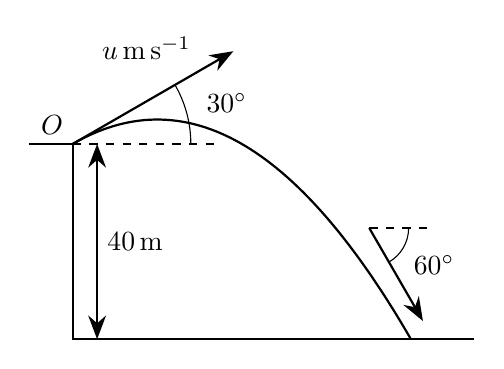
\begin{tikzpicture}[x=0.062cm, y=0.062cm]
\def\g{10}            % shape uses g = 10, so u = 20
\def\spd{20}          % u
\def\ang{30}          % angle of projection
\def\hgt{40}          % height of cliff
\def\velLen{38}       % drawn length of the initial-velocity arrow
\def\impLen{22}       % drawn length of the impact-velocity arrow
\def\impOff{4}        % offset of the impact arrow from the path (outer side)
\def\impGap{2}        % impact arrow stops this far short of the ground
\def\impRay{12}       % dashed horizontal at the tail of the impact arrow
\def\refLen{30}       % dashed horizontal reference ray at O
\def\cliffTop{9}      % visible cliff top behind O
\def\groundPad{13}    % ground beyond the landing point
\def\dimOff{5}        % offset of the 40 m dimension line from the cliff face
\pgfmathsetmacro{\ux}{\spd*cos(\ang)}
\pgfmathsetmacro{\uy}{\spd*sin(\ang)}
\pgfmathsetmacro{\tLand}{(\uy+sqrt(\uy*\uy+2*\g*\hgt))/\g}
\pgfmathsetmacro{\xLand}{\ux*\tLand}
\pgfmathsetmacro{\impAng}{atan2(\uy-\g*\tLand,\ux)}

\coordinate (O) at (0,0);
\coordinate (H) at (\refLen,0);
\coordinate (U) at (\ang:\velLen);
\coordinate (F) at (0,-\hgt);
\coordinate (L) at (\xLand,-\hgt);
\coordinate (R) at ($(L)+(\groundPad,0)$);
\coordinate (T) at ($(L)+(\impAng+90:\impOff)+(\impAng+180:\impGap)$);
\coordinate (S) at ($(T)+(\impAng+180:\impLen)$);
\coordinate (SH) at ($(S)+(\impRay,0)$);
\coordinate (D0) at (\dimOff,0);
\coordinate (D1) at (\dimOff,-\hgt);

\draw[thick, black] (-\cliffTop,0) -- (O) -- (F) -- (R);
\draw[dashed, black] (O) -- (H);
\draw[thick, black, variable=\t, domain=0:\tLand, samples=150]
  plot ({\ux*\t}, {\uy*\t-0.5*\g*\t*\t});

\draw[-{Stealth[length=3mm]}, thick, black] (O) -- (U)
  node[pos=0.8, above left] {$u\,\mathrm{m\,s^{-1}}$};
\pic["$30^\circ$", draw, angle radius=15mm, angle eccentricity=1.35] {angle=H--O--U};

\draw[dashed, black] (S) -- (SH);
\draw[-{Stealth[length=3mm]}, thick, black] (S) -- (T);
\pic["$60^\circ$", draw, angle radius=5mm, angle eccentricity=1.9] {angle=T--S--SH};

\draw[{Stealth[length=3mm]}-{Stealth[length=3mm]}, thick, black] (D0) -- (D1)
  node[midway, right] {$40\,\mathrm{m}$};

\node[above left] at (O) {$O$};
\end{tikzpicture}
\end{djsSolutionFigure}

Take horizontal motion away from the cliff and vertical motion upwards as positive. Use \(g=9.8\,\mathrm{m\,s^{-2}}\), and let \(t\) be the time taken to reach the ground.

The initial horizontal and vertical velocity components are
\[
v_{x0}=u\cos30^\circ=\dfrac{\sqrt{3}u}{2},
\qquad
v_{y0}=u\sin30^\circ=\dfrac{u}{2}
\]

There is no horizontal acceleration, so the horizontal velocity remains \(\frac{\sqrt{3}u}{2}\). Since this is positive, the impact direction perpendicular to the initial direction must be \(60^\circ\) below the horizontal. Hence the vertical velocity immediately before impact is
\begin{align*}
v_y&=-v_x\tan60^\circ\\
&=-\dfrac{\sqrt{3}u}{2}\times\sqrt{3}\\
&=-\dfrac{3u}{2}
\end{align*}

The constant acceleration formula is
\[
v^2=v_0^2+2as
\]

Applying this to the vertical motion, with initial velocity \(\frac{u}{2}\), acceleration \(-g\) and displacement \(-40\,\mathrm{m}\):
\begin{align*}
\left(-\dfrac{3u}{2}\right)^2
&=\left(\dfrac{u}{2}\right)^2+2(-g)(-40)\\
\dfrac{9u^2}{4}-\dfrac{u^2}{4}&=80g\\
2u^2&=80g\\
u^2&=40g=392
\end{align*}

The initial speed is positive, so
\[
u=14\sqrt{2}\,\mathrm{m\,s^{-1}}
\]

The constant acceleration formula is
\[
v=v_0+at
\]

Applying this to the vertical motion:
\begin{align*}
-\dfrac{3u}{2}&=\dfrac{u}{2}-gt\\
gt&=2u\\
t&=\dfrac{2u}{g}
=\dfrac{2\times14\sqrt{2}}{9.8}
=\dfrac{20\sqrt{2}}{7}\,\mathrm{s}
\end{align*}

\par\medskip\noindent\textbf{Final answers with \(g = 10\):} \(u = 20\,\mathrm{m\,s^{-1}}\);\quad \(t = 4\,\mathrm{s}\)
\end{djsSolution}

\newpage

% ---- Question 2 ----
\questionitem
% [Source: _QBT___Solns__Projectile_Motion, Q2]

A particle $P$ is projected from a point $O$, which is $30\,\mathrm{m}$ above horizontal ground, with speed $u\,\mathrm{m\,s^{-1}}$ at an angle $\theta$ above the horizontal, where $0<\theta<90^\circ$. \\
The particle moves freely under gravity and lands on the ground at a horizontal distance of $40\,\mathrm{m}$ from $O$. \\

The velocity of $P$ immediately before it lands is perpendicular to its initial velocity. \\

Find $u$ and $\theta$, giving the angle to one decimal place. \marks{8} \\

\vspace*{10pt}

\begin{djsSolution}
\begin{djsSolutionFigure}
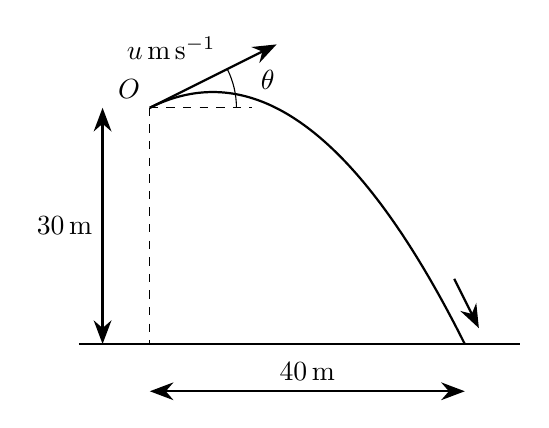
\begin{tikzpicture}[x=0.1cm, y=0.1cm]
\def\g{10}            % shape uses g = 10
\def\hgt{30}          % height of O above the ground
\def\range{40}        % horizontal distance to the landing point
\def\tanTh{0.5}       % tan(theta), from the solution
\def\velLen{18}       % drawn length of the initial-velocity arrow
\def\impLen{7}        % drawn length of the impact-velocity arrow
\def\impOff{2.5}      % offset of the impact arrow off the curve (outer side)
\def\impGap{1}        % impact arrow stops this far short of the landing point
\def\refLen{13}       % dashed horizontal reference ray at O
\def\groundL{9}       % ground to the left of O
\def\groundR{7}       % ground beyond the landing point
\def\dimOffH{6}       % offset of the 30 m dimension line left of O
\def\dimDrop{6}      % drop of the 40 m dimension line below the ground
\pgfmathsetmacro{\ang}{atan(\tanTh)}
\pgfmathsetmacro{\spd}{sqrt(\range*\g*\tanTh)}   % u^2 = 40 g tan(theta)
\pgfmathsetmacro{\ux}{\spd*cos(\ang)}
\pgfmathsetmacro{\uy}{\spd*sin(\ang)}
\pgfmathsetmacro{\tLand}{\range/\ux}
\pgfmathsetmacro{\impAng}{atan2(\uy-\g*\tLand,\ux)}

\coordinate (O) at (0,0);
\coordinate (H) at (\refLen,0);
\coordinate (U) at (\ang:\velLen);
\coordinate (F) at (0,-\hgt);
\coordinate (L) at (\range,-\hgt);
\coordinate (VE) at ($(L)+(\impAng+90:\impOff)+(\impAng:-\impGap)$);
\coordinate (VS) at ($(VE)+(\impAng:-\impLen)$);
\coordinate (GL) at ($(F)+(-\groundL,0)$);
\coordinate (GR) at ($(L)+(\groundR,0)$);
\coordinate (A0) at (-\dimOffH,0);
\coordinate (A1) at (-\dimOffH,-\hgt);
\coordinate (B0) at ($(F)+(0,-\dimDrop)$);
\coordinate (B1) at ($(L)+(0,-\dimDrop)$);

\draw[thick, black] (GL) -- (GR);
\draw[dashed, black] (O) -- (F);
\draw[dashed, black] (O) -- (H);
\draw[thick, black, variable=\t, domain=0:\tLand, samples=150]
  plot ({\ux*\t}, {\uy*\t-0.5*\g*\t*\t});

\draw[-{Stealth[length=3mm]}, thick, black] (O) -- (U)
  node[pos=0.6, above left] {$u\,\mathrm{m\,s^{-1}}$};
\pic["$\theta$", draw, angle radius=11mm, angle eccentricity=1.4] {angle=H--O--U};

\draw[-{Stealth[length=3mm]}, thick, black] (VS) -- (VE);

\draw[{Stealth[length=3mm]}-{Stealth[length=3mm]}, thick, black] (A0) -- (A1)
  node[midway, left] {$30\,\mathrm{m}$};
\draw[{Stealth[length=3mm]}-{Stealth[length=3mm]}, thick, black] (B0) -- (B1)
  node[midway, above] {$40\,\mathrm{m}$};

\node[above left] at (O) {$O$};
\end{tikzpicture}
\end{djsSolutionFigure}

Take horizontal motion away from \(O\) and vertical motion upwards as positive. Use \(g=9.8\,\mathrm{m\,s^{-2}}\). Let the flight time be \(T\,\mathrm{s}\) and the signed vertical velocity immediately before landing be \(v_y\,\mathrm{m\,s^{-1}}\).

The horizontal velocity remains \(u\cos\theta\). The constant acceleration formula is
\[
s=v_0t+\frac12at^2
\]

Applying this horizontally, with \(a=0\), gives
\[
40=u\cos\theta\,T
\quad\Longrightarrow\quad
T=\frac{40}{u\cos\theta}
\]

The final velocity points forwards and downwards, perpendicular to the initial velocity, so it makes an angle of \(90^\circ-\theta\) below the horizontal. Hence
\[
\frac{v_y}{u\cos\theta}=-\tan(90^\circ-\theta)=-\cot\theta
\quad\Longrightarrow\quad
v_y=-u\cos\theta\cot\theta
\]

The constant acceleration formula is
\[
s=\frac12(v_0+v)t
\]

Applying this vertically:
\begin{align*}
-30&=\frac12(u\sin\theta+v_y)T\\
&=\frac12\left(u\sin\theta-u\cos\theta\cot\theta\right)
\frac{40}{u\cos\theta}\\
&=20(\tan\theta-\cot\theta)
\end{align*}

Multiplying by \(\tan\theta\) and rearranging:
\begin{align*}
2\tan^2\theta+3\tan\theta-2&=0\\
(2\tan\theta-1)(\tan\theta+2)&=0
\end{align*}

Since \(0<\theta<90^\circ\), we reject \(\tan\theta=-2\), giving
\[
\tan\theta=\frac12
\quad\Longrightarrow\quad
\theta=\arctan\left(\frac12\right)\approx26.6^\circ
\qquad\text{(1 d.p.)}
\]

The constant acceleration formula is
\[
v=v_0+at
\]

Applying this vertically:
\begin{align*}
v_y&=u\sin\theta-gT\\
gT&=u\sin\theta+u\cos\theta\cot\theta\\
&=\frac{u(\sin^2\theta+\cos^2\theta)}{\sin\theta}
=\frac{u}{\sin\theta}
\end{align*}

Substituting \(T=\frac{40}{u\cos\theta}\):
\begin{align*}
\frac{40g}{u\cos\theta}&=\frac{u}{\sin\theta}\\
u^2&=40g\tan\theta=20g\\
u&=\sqrt{20\times9.8}=14\,\mathrm{m\,s^{-1}}
\end{align*}

\par\medskip\noindent\textbf{Final answers with \(g = 10\):} \(u=14.1\,\mathrm{m\,s^{-1}}\)
\end{djsSolution}

\newpage

% ---- Question 3 ----
\questionitem
% [Source: _QBT___Solns__Projectile_Motion, Q3]

A particle $P$ is projected from a point $O$ at time $t=0$ with speed $u\,\mathrm{m\,s^{-1}}$ at an angle $\theta$ above the horizontal, where $0<\theta<90^\circ$. \\
The particle moves freely under gravity, with $g=10\,\mathrm{m\,s^{-2}}$. \\
After $6$ seconds, its speed is $\sqrt{5}u\,\mathrm{m\,s^{-1}}$. \\

\begin{enumerate}[label=\textbf{(\alph*)}]
\item Show that
\[
u^2+30u\sin\theta-900=0
\] \marks[-20pt]{3}
\item At time $t=6\,\mathrm{s}$, the particle is at a point $A$ below the horizontal level of $O$. \\
The displacement vector $\overrightarrow{OA}$ is perpendicular to the initial velocity of $P$. \\
Find the exact value of $u$, the value of $\theta$, and the exact distance $OA$. \marks{6} \\
\end{enumerate}

\vspace*{10pt}

\begin{djsSolution}
\begin{djsSolutionFigure}
\begin{tikzpicture}[x=0.05cm,y=0.05cm]
\def\ang{45}
\def\g{10}
\def\T{6}
\def\velocityArrowLen{32}
\def\angleRayLen{20}
\def\refLeft{-8}
\def\refRight{8}
\def\rightMark{2.5mm}
\pgfmathsetmacro{\spd}{15*sqrt(2)}
\pgfmathsetmacro{\ux}{\spd*cos(\ang)}
\pgfmathsetmacro{\uy}{\spd*sin(\ang)}
\pgfmathsetmacro{\xA}{\ux*\T}
\pgfmathsetmacro{\yA}{\uy*\T-0.5*\g*\T*\T}

\coordinate (O) at (0,0);
\coordinate (H) at (\angleRayLen,0);
\coordinate (U) at (\ang:\velocityArrowLen);
\coordinate (A) at (\xA,\yA);
\coordinate (R1) at ($(O)!\rightMark!(U)$);
\coordinate (R2) at ($(O)!\rightMark!(A)$);
\coordinate (R3) at ($(R1)+(R2)-(O)$);

\draw[dashed, black] (\refLeft,0) -- (\xA+\refRight,0);
\draw[thick, black, variable=\t, domain=0:\T, samples=150]
  plot ({\ux*\t}, {\uy*\t-0.5*\g*\t*\t});
\draw[dashed, black] (O) -- (A);
\draw[black] (R1) -- (R3) -- (R2);

\draw[-{Stealth[length=3mm]}, thick, black] (O) -- (U)
  node[pos=0.8, above left] {$u\,\mathrm{m\,s^{-1}}$};
\pic["$\theta$", draw, angle radius=7mm, angle eccentricity=1.35] {angle=H--O--U};

\fill[black] (O) circle (1.2pt);
\fill[black] (A) circle (1.2pt);
\node[below left] at (O) {$O$};
\node[right=2pt] at (A) {$A$};
\end{tikzpicture}
\end{djsSolutionFigure}

\begin{enumerate}[label=\textbf{(\alph*)}, start=1]
\item Take horizontal motion to the right and vertical motion upwards as positive. The acceleration components are \(0\) and \(-10\,\mathrm{m\,s^{-2}}\).

The constant acceleration formula is
\[
v=v_0+at
\]

Applying this, the velocity components after \(6\) seconds are
\[
v_x=u\cos\theta,\qquad v_y=u\sin\theta-10(6)=u\sin\theta-60
\]

The square of the speed is \(v_x^2+v_y^2\), so
\begin{align*}
(u\cos\theta)^2+(u\sin\theta-60)^2&=(\sqrt{5}u)^2\\
u^2(\cos^2\theta+\sin^2\theta)-120u\sin\theta+3600&=5u^2\\
4u^2+120u\sin\theta-3600&=0\\
u^2+30u\sin\theta-900&=0
\end{align*}

\item The constant acceleration formula is
\[
s=v_0t+\frac12at^2
\]

Applying this, the horizontal and vertical displacements after \(6\) seconds are
\begin{align*}
x&=(u\cos\theta)(6)=6u\cos\theta\\
y&=(u\sin\theta)(6)+\frac12(-10)(6^2)=6u\sin\theta-180
\end{align*}

Perpendicular vectors have zero scalar product. Hence the displacement and initial velocity satisfy
\begin{align*}
\begin{pmatrix}6u\cos\theta\\6u\sin\theta-180\end{pmatrix}
\cdot\begin{pmatrix}u\cos\theta\\u\sin\theta\end{pmatrix}&=0\\
6u^2\cos^2\theta+6u^2\sin^2\theta-180u\sin\theta&=0\\
6u^2-180u\sin\theta&=0
\end{align*}

Since \(u>0\), dividing by \(6u\) gives
\[
u=30\sin\theta
\]

Substituting \(30u\sin\theta=u^2\) into the result from part (a):
\begin{align*}
u^2+u^2-900&=0\\
u^2&=450\\
u&=15\sqrt{2}\,\mathrm{m\,s^{-1}}
\end{align*}

Using \(u=30\sin\theta\) and \(0<\theta<90^\circ\):
\begin{align*}
\sin\theta&=\frac{15\sqrt{2}}{30}=\frac{1}{\sqrt{2}}\\
\theta&=45^\circ
\end{align*}

The displacement is therefore
\[
\overrightarrow{OA}
=\begin{pmatrix}6(15\sqrt{2})\cos45^\circ\\6(15\sqrt{2})\sin45^\circ-180\end{pmatrix}\,\mathrm{m}
=\begin{pmatrix}90\\-90\end{pmatrix}\,\mathrm{m}
\]

Its magnitude gives the distance:
\[
OA=\sqrt{90^2+(-90)^2}=90\sqrt{2}\,\mathrm{m}
\]

\end{enumerate}
\end{djsSolution}

\newpage

% ---- Question 4 ----
\questionitem
% [Source: _QBT___Solns__Projectile_Motion, Q4]

At time $t=0$, a particle $P$ is projected from a point $O$ on horizontal ground with speed $26\,\mathrm{m\,s^{-1}}$ at an angle $\alpha$ above the horizontal, where $\sin\alpha=\frac{12}{13}$. \\
A point $A$ on the ground lies $40\,\mathrm{m}$ from $O$ in the direction of the horizontal motion of $P$. \\

At time $t=T\,\mathrm{s}$, where $T>0$, a second particle $Q$ is projected vertically upwards from $A$ with speed $22\,\mathrm{m\,s^{-1}}$. \\
The particles collide while $Q$ is travelling upwards. \\
Before the collision, both particles move freely under gravity. \\
Neglect air resistance throughout. \\

\begin{enumerate}[label=\textbf{(\alph*)}]
\item Find the time at which the particles collide and their height above the ground at that instant. \marks{2} \\
\item Find the exact value of $T$. \marks{5} \\
\item Immediately after the collision, the speed of $P$ is $v\,\mathrm{m\,s^{-1}}$ and its direction of motion is above the horizontal. \\
Its horizontal velocity component is unchanged by the collision, and it subsequently moves freely under gravity. \\
Find its greatest height above the ground in terms of $v$. Hence find the least possible value of $v$ for $P$ to reach a height of $40\,\mathrm{m}$ above the ground. \marks{4} \\
\end{enumerate}

\vspace*{10pt}

\begin{djsSolution}
\begin{djsSolutionFigure}
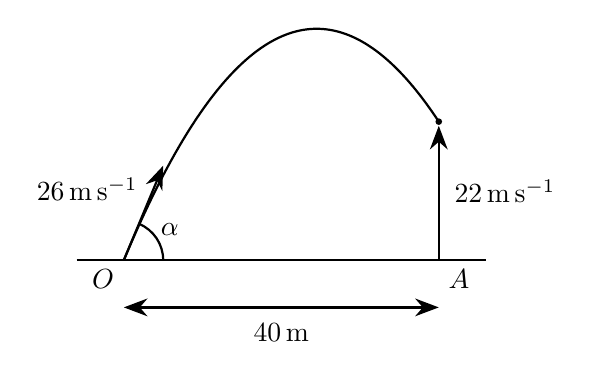
\begin{tikzpicture}[x=1mm, y=1mm]
\def\speedP{26}
\def\sinAlpha{12/13}
\def\dOA{40}
\def\grav{9.8}
\def\velArrowLen{13}
\def\groundPad{6}
\def\dimDrop{6}
\pgfmathsetmacro{\ang}{asin(\sinAlpha)}
\pgfmathsetmacro{\ux}{\speedP*cos(\ang)}
\pgfmathsetmacro{\uy}{\speedP*sin(\ang)}
\pgfmathsetmacro{\tC}{\dOA/\ux}
\pgfmathsetmacro{\yC}{\uy*\tC - 0.5*\grav*\tC*\tC}

\coordinate (O) at (0,0);
\coordinate (A) at (\dOA,0);
\coordinate (C) at (\dOA,\yC);
\coordinate (H) at (\velArrowLen,0);
\coordinate (U) at (\ang:\velArrowLen);
\coordinate (D0) at ($(O)+(0,-\dimDrop)$);
\coordinate (D1) at ($(A)+(0,-\dimDrop)$);

\draw[thick, black] (-\groundPad,0) -- (\dOA+\groundPad,0);
\draw[thick, black, domain=0:\tC, samples=150, variable=\t]
  plot ({\ux*\t}, {\uy*\t - 0.5*\grav*\t*\t});

\draw[-{Stealth[length=3mm]}, thick, black] (O) -- (U)
  node[pos=0.75, left=2pt] {$26\,\mathrm{m\,s^{-1}}$};
\pic["$\alpha$", draw, thick, angle radius=5mm, angle eccentricity=1.4] {angle=H--O--U};

\draw[-{Stealth[length=3mm]}, thick, black, shorten >=1.5pt] (A) -- (C)
  node[midway, right=2pt] {$22\,\mathrm{m\,s^{-1}}$};
\fill[black] (C) circle (1.2pt);

\draw[{Stealth[length=3mm]}-{Stealth[length=3mm]}, thick, black] (D0) -- (D1)
  node[midway, below=2pt] {$40\,\mathrm{m}$};

\node[below left] at (O) {$O$};
\node[below right] at (A) {$A$};
\end{tikzpicture}
\end{djsSolutionFigure}

Take horizontal motion from \(O\) towards \(A\) and vertical motion upwards as positive. Use \(g=9.8\,\mathrm{m\,s^{-2}}\).

\begin{enumerate}[label=\textbf{(\alph*)}, start=1]
\item Since \(\alpha\) is above the horizontal, \(\cos\alpha=\frac{5}{13}\). The horizontal and vertical components of the initial velocity of \(P\) are \(26\times\frac{5}{13}=10\,\mathrm{m\,s^{-1}}\) and \(26\times\frac{12}{13}=24\,\mathrm{m\,s^{-1}}\).

The collision occurs directly above \(A\). The constant acceleration formula is
\[
s=v_0t+\frac12at^2
\]

Applying this horizontally, where the acceleration is zero, and then vertically:
\begin{align*}
40&=10t \quad\Longrightarrow\quad t=4\,\mathrm{s} \\
\text{Height}&=24(4)-\frac12(9.8)(4^2)=17.6\,\mathrm{m}
\end{align*}

\item At the collision, \(Q\) has been moving for \((4-T)\,\mathrm{s}\). Applying the displacement formula from part (a) to \(Q\):
\begin{align*}
17.6&=22(4-T)-4.9(4-T)^2 \\
17.6&=9.6+17.2T-4.9T^2 \\
49T^2-172T+80&=0 \\
T&=\frac{86\pm2\sqrt{869}}{49}
\end{align*}

The constant acceleration formula is
\[
v=v_0+at
\]

Applying this to \(Q\), the condition that \(Q\) is travelling upwards gives
\begin{align*}
22-9.8(4-T)&>0 \\
T&>\frac{86}{49}
\end{align*}

Therefore the required root is
\[
T=\frac{86+2\sqrt{869}}{49}\,\mathrm{s}
\]

\item Let \(w>0\) be the upward velocity component of \(P\) immediately after the collision. Its horizontal component remains \(10\,\mathrm{m\,s^{-1}}\), so
\[
w^2+10^2=v^2\quad\Longrightarrow\quad w^2=v^2-100
\]

Let the greatest height above the ground be \(H\,\mathrm{m}\). At this height the vertical velocity is zero. The constant acceleration formula is
\[
v_y^2=v_{y0}^2+2as
\]

Applying this to the vertical motion after the collision, with \(v_{y0}=w\):
\begin{align*}
0&=w^2-2(9.8)(H-17.6) \\
H&=17.6+\frac{v^2-100}{19.6}
\end{align*}

Thus the greatest height is
\[
\left(\frac{88}{5}+\frac{5(v^2-100)}{98}\right)\,\mathrm{m}
\]

Hence, for \(P\) to reach \(40\,\mathrm{m}\):
\begin{align*}
17.6+\frac{v^2-100}{19.6}&\geq40 \\
v^2&\geq100+19.6(40-17.6)=\frac{13476}{25}
\end{align*}

Since \(v\) is positive, the least possible speed is
\[
v_{\min}=\frac{2\sqrt{3369}}{5}\,\mathrm{m\,s^{-1}}
\]

\end{enumerate}
\par\medskip\noindent\textbf{Final answers with \(g = 10\):} (a) height \(16\,\mathrm{m}\);\quad (b) \(T=\frac{9+\sqrt{41}}{5}\,\mathrm{s}\);\quad (c) greatest height \(\left(11+\frac{v^2}{20}\right)\,\mathrm{m}\), \(v_{\min}=2\sqrt{145}\,\mathrm{m\,s^{-1}}\)
\end{djsSolution}

\newpage

% ---- Question 5 ----
\questionitem
% [Source: _QBT___Solns__Projectile_Motion, Q5]

A particle $P$ is projected from a point $A$ which is vertically above a fixed point $O$ on horizontal ground, with $OA=h$. \\
Its initial velocity is $u(4\mathbf{i}+3\mathbf{j})$, where $u>0$ and $h>0$. \\
The unit vectors $\mathbf{i}$ and $\mathbf{j}$ are horizontal and vertically upwards respectively. \\
The particle moves freely under gravity, with constant acceleration $-g\mathbf{j}$. \\

At time $t=0$, the particle leaves $A$. \\
Its position vector relative to $O$ at time $t$ is $\mathbf{r}=x\mathbf{i}+y\mathbf{j}$. \\

\begin{enumerate}[label=\textbf{(\alph*)}]
\item Starting from an expression for $\ddot{\mathbf{r}}$, use integration to obtain $\mathbf{r}$ in terms of $t$, $u$, $h$ and $g$. \marks{4} \\
\item Eliminate $t$ to obtain the Cartesian equation of the path of $P$. \marks{3} \\
\item Hence find the maximum height of $P$ above the ground, in terms of $u$, $h$ and $g$. \marks{3} \\
\item When $P$ first strikes the ground, its velocity is perpendicular to its initial velocity. Determine $h$ in terms of $u$ and $g$. \marks{4} \\
\end{enumerate}

\vspace*{10pt}

\begin{djsSolution}
\begin{djsSolutionFigure}
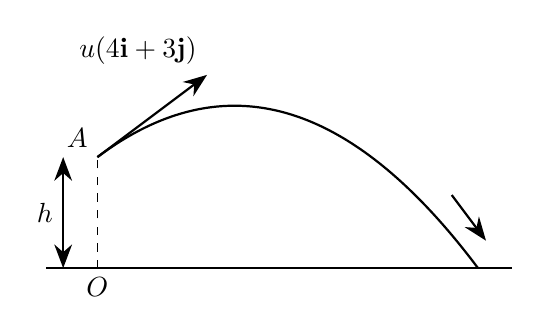
\begin{tikzpicture}[x=0.145cm, y=0.145cm]
\def\spd{1}         % u (symbolic shape: u = g = 1)
\def\grav{1}        % g
\def\vx{4}          % initial velocity u(4i + 3j)
\def\vy{3}
\def\velLen{12}     % drawn length of the initial-velocity arrow
\def\impLen{5}      % drawn length of the impact-velocity arrow
\def\impGap{1.5}    % impact arrow stops this far short of the landing point
\def\impOff{2}      % impact arrow offset from the curve, on its outer side
\def\dimOff{3}      % offset of the h dimension line to the left of OA
\def\groundLeft{1.5}% ground beyond the dimension line
\def\groundPad{3}   % ground beyond the landing point
\pgfmathsetmacro{\launchAng}{atan2(\vy,\vx)}
\pgfmathsetmacro{\tLand}{(\vx*\vx+\vy*\vy)*\spd/(\vy*\grav)}
\pgfmathsetmacro{\hgt}{0.5*\grav*\tLand*\tLand-\vy*\spd*\tLand}
\pgfmathsetmacro{\xLand}{\vx*\spd*\tLand}
\pgfmathsetmacro{\impAng}{atan2(\vy*\spd-\grav*\tLand,\vx*\spd)}

\coordinate (O) at (0,0);
\coordinate (A) at (0,\hgt);
\coordinate (L) at (\xLand,0);
\coordinate (Vend) at ($(L)+(\impAng+180:\impGap)+(\impAng+90:\impOff)$);
\coordinate (Vstart) at ($(Vend)+(\impAng+180:\impLen)$);
\coordinate (D0) at (-\dimOff,0);
\coordinate (D1) at (-\dimOff,\hgt);

\draw[thick, black] ({-\dimOff-\groundLeft},0) -- ({\xLand+\groundPad},0);
\draw[dashed, black] (O) -- (A);
\draw[thick, black, domain=0:\tLand, samples=150]
  plot ({\vx*\spd*\x}, {\hgt+\vy*\spd*\x-0.5*\grav*\x*\x});

\draw[-{Stealth[length=3mm]}, thick, black] (A) -- ++(\launchAng:\velLen)
  node[above left] {$u(4\mathbf{i}+3\mathbf{j})$};
\draw[-{Stealth[length=3mm]}, thick, black] (Vstart) -- (Vend);

\draw[{Stealth[length=3mm]}-{Stealth[length=3mm]}, thick, black] (D0) -- (D1)
  node[midway, left] {$h$};

\node[below] at (O) {$O$};
\node[above left] at (A) {$A$};
\end{tikzpicture}
\end{djsSolutionFigure}

\begin{enumerate}[label=\textbf{(\alph*)}, start=1]
\item The acceleration is
\[
\ddot{\mathbf r}=-g\mathbf j,
\qquad \ddot{x}=0,\qquad \ddot{y}=-g
\]

Integrating each component with respect to \(t\):
\[
\dot{x}=c_1,\qquad \dot{y}=-gt+c_2
\]

The initial velocity is \(4u\mathbf i+3u\mathbf j\), so \(c_1=4u\) and \(c_2=3u\). Integrating again:
\[
x=4ut+c_3,\qquad y=3ut-\dfrac12gt^2+c_4
\]

At \(t=0\), the particle is at \(A\), so \(x=0\) and \(y=h\). Hence \(c_3=0\) and \(c_4=h\), giving
\[
\mathbf r=4ut\mathbf i+\left(h+3ut-\dfrac12gt^2\right)\mathbf j
\]

\item From the horizontal component in part (a):
\[
x=4ut\quad\Longrightarrow\quad t=\dfrac{x}{4u}
\]

Substituting into the vertical component:
\begin{align*}
y&=h+3u\left(\dfrac{x}{4u}\right)-\dfrac12g\left(\dfrac{x}{4u}\right)^2\\
&=h+\dfrac{3x}{4}-\dfrac{gx^2}{32u^2}
\end{align*}

\item Completing the square in the equation from part (b):
\begin{align*}
y&=h-\dfrac{g}{32u^2}\left(x^2-\dfrac{24u^2}{g}x\right)\\
&=h-\dfrac{g}{32u^2}\left[\left(x-\dfrac{12u^2}{g}\right)^2-\dfrac{144u^4}{g^2}\right]\\
&=h+\dfrac{9u^2}{2g}-\dfrac{g}{32u^2}\left(x-\dfrac{12u^2}{g}\right)^2
\end{align*}

Since the squared term is non-negative and \(g>0\), the maximum occurs at \(x=\frac{12u^2}{g}>0\). The maximum height above the ground is therefore
\[
h+\dfrac{9u^2}{2g}
\]

\item The horizontal velocity remains \(4u\). Let the vertical velocity when the particle strikes the ground be \(v_y\). Perpendicular vectors have zero scalar product, so the two velocities satisfy
\begin{align*}
(4u)(4u)+(3u)v_y&=0\\
v_y&=-\dfrac{16u}{3}
\end{align*}

The constant acceleration formula is
\[
v^2=v_0^2+2as
\]

For the vertical motion, \(v=v_y\), \(v_0=3u\), \(a=-g\) and the displacement to the ground is \(s=-h\). Substituting:
\begin{align*}
\left(-\dfrac{16u}{3}\right)^2&=(3u)^2+2(-g)(-h)\\
\dfrac{256u^2}{9}&=9u^2+2gh\\
2gh&=\dfrac{175u^2}{9}\\
h&=\dfrac{175u^2}{18g}
\end{align*}

\end{enumerate}
\end{djsSolution}

\newpage

% ---- Question 6 ----
\questionitem
% [Source: _QBT___Solns__Projectile_Motion, Q6]

\begin{figure}[H]
    \centering
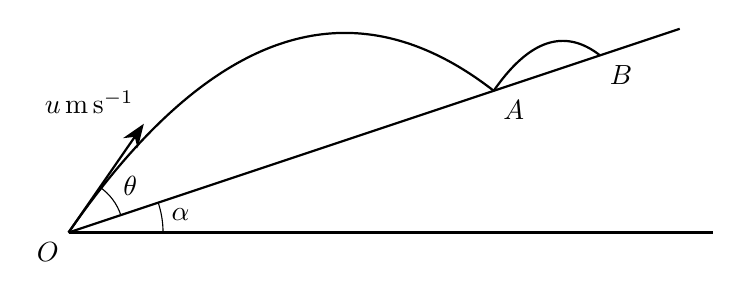
\begin{tikzpicture}[x=0.12cm,y=0.12cm]
\def\grav{10}
\def\launchSpeed{25}
\def\tanAlpha{1/3}
\def\tanTheta{3/4}
\def\restitution{0.5}
\def\arrowLength{14}
\def\extension{1.15}
\pgfmathsetmacro{\alph}{atan(\tanAlpha)}
\pgfmathsetmacro{\thet}{atan(\tanTheta)}
\pgfmathsetmacro{\gs}{\grav*sin(\alph)}
\pgfmathsetmacro{\gn}{\grav*cos(\alph)}
\pgfmathsetmacro{\us}{\launchSpeed*cos(\thet)}
\pgfmathsetmacro{\un}{\launchSpeed*sin(\thet)}
\pgfmathsetmacro{\firstTime}{2*\un/\gn}
\pgfmathsetmacro{\sA}{\us*\firstTime-\gs*\firstTime^2/2}
\pgfmathsetmacro{\vs}{\us-\gs*\firstTime}
\pgfmathsetmacro{\vn}{\restitution*\un}
\pgfmathsetmacro{\secondTime}{2*\vn/\gn}
\pgfmathsetmacro{\sB}{\sA+\vs*\secondTime-\gs*\secondTime^2/2}
\coordinate (O) at (0,0);
\coordinate (H) at ({\extension*\sB},0);
\draw[thick,black] (O) -- (H);
\begin{scope}[rotate=\alph]
  \coordinate (A) at (\sA,0);
  \coordinate (B) at (\sB,0);
  \coordinate (S) at ({\extension*\sB},0);
  \coordinate (V) at (\thet:\arrowLength);
  \draw[thick,black] (O) -- (S);
  \draw[thick,black,domain=0:\firstTime,samples=120,variable=\t]
    plot ({\us*\t-\gs*\t^2/2},{\un*\t-\gn*\t^2/2});
  \draw[thick,black,domain=0:\secondTime,samples=100,variable=\t]
    plot ({\sA+\vs*\t-\gs*\t^2/2},{\vn*\t-\gn*\t^2/2});
  \draw[-{Stealth[length=3mm]},thick,black] (O) -- (V)
    node[above left] {$u\,\mathrm{m\,s^{-1}}$};
\end{scope}
\pic["$\alpha$",draw,angle radius=12mm,angle eccentricity=1.2] {angle=H--O--S};
\pic["$\theta$",draw,angle radius=7mm,angle eccentricity=1.4] {angle=S--O--V};
\node[below left] at (O) {$O$};
\node[below right] at (A) {$A$};
\node[below right] at (B) {$B$};
\end{tikzpicture}
\end{figure}


A small ball $P$ is projected from a point $O$ at the foot of a smooth plane inclined at an angle $\alpha$ to the horizontal, where $\tan\alpha=\frac{1}{3}$. \\
Its initial speed is $u\,\mathrm{m\,s^{-1}}$, and its initial velocity makes an angle $\theta$ above the plane, where $\tan\theta=\frac{3}{4}$. \\

The ball first strikes the plane at $A$, where $OA=15\sqrt{10}\,\mathrm{m}$. \\
Its motion takes place in the vertical plane containing a line of greatest slope of the inclined plane, and air resistance is negligible. \\

\begin{enumerate}[label=\textbf{(\alph*)}]
\item Find $u$ and the components of the ball's velocity parallel and perpendicular to the plane immediately before impact at $A$. State the direction of each component. \marks{8} \\
\end{enumerate}
The ball rebounds from the plane at $A$ and next strikes it at $B$, further up the plane, where
\[
AB=\frac{15\sqrt{10}}{4}\,\mathrm{m}
\] \\
\begin{enumerate}[label=\textbf{(\alph*)}, resume]
\item Find the coefficient of restitution between the ball and the plane, explaining why any other algebraic solution must be rejected. \marks{8} \\
\end{enumerate}

\vspace*{10pt}

\begin{djsSolution}
\begin{enumerate}[label=\textbf{(\alph*)}, start=1]
\item Take horizontal motion to the right and vertical motion upwards as positive. Use \(g=9.8\,\mathrm{m\,s^{-2}}\).

From the given tangents:
\[
\sin\alpha=\frac{1}{\sqrt{10}},\qquad \cos\alpha=\frac{3}{\sqrt{10}},\qquad
\sin\theta=\frac35,\qquad \cos\theta=\frac45
\]

The launch angle above the horizontal is \(\alpha+\theta\), so the initial horizontal and vertical velocity components are
\begin{align*}
v_{x0}&=u\cos(\alpha+\theta)
=u\left(\frac{3}{\sqrt{10}}\times\frac45-\frac{1}{\sqrt{10}}\times\frac35\right)
=\frac{9u}{5\sqrt{10}}\\
v_{y0}&=u\sin(\alpha+\theta)
=u\left(\frac{1}{\sqrt{10}}\times\frac45+\frac{3}{\sqrt{10}}\times\frac35\right)
=\frac{13u}{5\sqrt{10}}
\end{align*}

The horizontal and vertical displacements from \(O\) to \(A\) are
\begin{align*}
x_A&=OA\cos\alpha=15\sqrt{10}\times\frac{3}{\sqrt{10}}=45\,\mathrm{m}\\
y_A&=OA\sin\alpha=15\sqrt{10}\times\frac{1}{\sqrt{10}}=15\,\mathrm{m}
\end{align*}

The constant acceleration formula is
\[
s=v_0t+\frac12at^2
\]

Let the flight time from \(O\) to \(A\) be \(t_A\). Applying this formula horizontally and vertically gives
\begin{align*}
45&=\frac{9u}{5\sqrt{10}}t_A
\quad\Longrightarrow\quad ut_A=25\sqrt{10}\\
15&=\frac{13u}{5\sqrt{10}}t_A-\frac12gt_A^2\\
15&=65-\frac12gt_A^2\\
t_A&=\frac{10}{\sqrt g}\,\mathrm{s}
\end{align*}

Hence the initial speed is
\[
u=\frac{25\sqrt{10}}{10/\sqrt g}=\frac52\sqrt{10g}\,\mathrm{m\,s^{-1}}
\]

The constant acceleration formula is
\[
v=v_0+at
\]

Immediately before impact, the horizontal and vertical components are therefore
\begin{align*}
v_x&=\frac{9u}{5\sqrt{10}}=\frac92\sqrt g\,\mathrm{m\,s^{-1}}\\
v_y&=\frac{13u}{5\sqrt{10}}-gt_A
=\frac{13}{2}\sqrt g-10\sqrt g
=-\frac72\sqrt g\,\mathrm{m\,s^{-1}}
\end{align*}

Resolving parallel to the plane, positive up the plane, and perpendicular to it, positive away from the plane:
\begin{align*}
v_{\parallel}&=v_x\cos\alpha+v_y\sin\alpha
=\frac{27\sqrt g-7\sqrt g}{2\sqrt{10}}
=\sqrt{10g}\,\mathrm{m\,s^{-1}}\\
v_{\perp}&=-v_x\sin\alpha+v_y\cos\alpha
=\frac{-9\sqrt g-21\sqrt g}{2\sqrt{10}}
=-\frac32\sqrt{10g}\,\mathrm{m\,s^{-1}}
\end{align*}

Using \(g=9.8\,\mathrm{m\,s^{-2}}\), the required speed and component magnitudes are
\begin{align*}
u&=\frac{35\sqrt2}{2}\,\mathrm{m\,s^{-1}}\approx24.7\,\mathrm{m\,s^{-1}}\\
\text{Parallel component}&=7\sqrt2\,\mathrm{m\,s^{-1}}\approx9.90\,\mathrm{m\,s^{-1}}\quad\text{up the plane}\\
\text{Perpendicular component}&=\frac{21\sqrt2}{2}\,\mathrm{m\,s^{-1}}\approx14.8\,\mathrm{m\,s^{-1}}\quad\text{towards the plane}
\end{align*}

\item Let the coefficient of restitution be \(e\). Since the plane is smooth, the parallel velocity component is unchanged by impact. The perpendicular component reverses direction and its magnitude is multiplied by \(e\). Thus, immediately after impact, the components are
\[
v_{\parallel}=\sqrt{10g}\,\mathrm{m\,s^{-1}},\qquad
v_{\perp}=\frac{3e}{2}\sqrt{10g}\,\mathrm{m\,s^{-1}}
\]

Take up the plane and away from the plane as positive. The corresponding acceleration components are \(-g\sin\alpha=-\frac{g}{\sqrt{10}}\) and \(-g\cos\alpha=-\frac{3g}{\sqrt{10}}\).

Let the flight time from \(A\) to \(B\) be \(t_B\). Using the displacement formula from part (a), the perpendicular displacement is zero, so
\begin{align*}
0&=\frac{3e}{2}\sqrt{10g}\,t_B-\frac{3g}{2\sqrt{10}}t_B^2\\
0&=\frac32t_B\left(e\sqrt{10g}-\frac{g}{\sqrt{10}}t_B\right)\\
t_B&=\frac{10e}{\sqrt g}\,\mathrm{s}
\end{align*}

Applying the same displacement formula parallel to the plane:
\begin{align*}
AB&=\sqrt{10g}\,t_B-\frac{g}{2\sqrt{10}}t_B^2\\
&=\sqrt{10g}\frac{10e}{\sqrt g}
-\frac{g}{2\sqrt{10}}\frac{100e^2}{g}\\
&=5\sqrt{10}(2e-e^2)\,\mathrm{m}
\end{align*}

Substituting the given distance:
\begin{align*}
\frac{15\sqrt{10}}4&=5\sqrt{10}(2e-e^2)\\
4e^2-8e+3&=0\\
(2e-1)(2e-3)&=0\\
e&=\frac12\quad\text{or}\quad e=\frac32
\end{align*}

A coefficient of restitution must satisfy \(0\leq e\leq1\), so \(\frac32\) is rejected. Therefore
\[
e=\frac12
\]

\end{enumerate}
\par\medskip\noindent\textbf{Final answers with \(g = 10\):} (a) \(u=25\,\mathrm{m\,s^{-1}}\), parallel component \(10\,\mathrm{m\,s^{-1}}\) up the plane, perpendicular component \(15\,\mathrm{m\,s^{-1}}\) towards the plane
\end{djsSolution}

\newpage

% ---- Question 7 ----
\questionitem
% [Source: _QBT___Solns__Projectile_Motion, Q7]

\begin{figure}[H]
    \centering
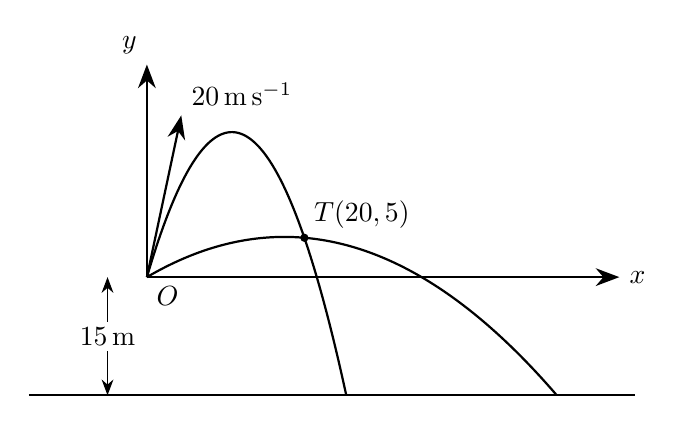
\begin{tikzpicture}[x=0.10cm,y=0.10cm]
\def\speed{20}
\def\grav{10}
\def\height{15}
\def\targetX{20}
\def\targetY{5}
\def\groundLeft{-15}
\def\groundRight{62}
\def\axisRight{60}
\def\axisTop{27}
\def\arrowAngle{78}
\def\arrowLength{21}
\def\dimOffset{5}
\pgfmathsetmacro{\lowAngle}{atan(2-sqrt(2))}
\pgfmathsetmacro{\highAngle}{atan(2+sqrt(2))}
\coordinate (O) at (0,0);
\coordinate (G) at (0,-\height);
\coordinate (T) at (\targetX,\targetY);
\coordinate (Dtop) at ($(O)+(-\dimOffset,0)$);
\coordinate (Dbottom) at ($(G)+(-\dimOffset,0)$);
\draw[thick,black] (\groundLeft,-\height) -- (\groundRight,-\height);
\foreach \ang in {\highAngle,\lowAngle} {
  \pgfmathsetmacro{\flight}{(\speed*sin(\ang)+sqrt((\speed*sin(\ang))^2+2*\grav*\height))/\grav}
  \draw[thick,black,domain=0:\flight,samples=120,variable=\t] plot ({\speed*cos(\ang)*\t},{\speed*sin(\ang)*\t-\grav*\t^2/2});
}
\draw[-{Stealth[length=3mm]},thick,black] (O) -- (\axisRight,0) node[right] {$x$};
\draw[-{Stealth[length=3mm]},thick,black] (O) -- (0,\axisTop) node[above left] {$y$};
\draw[-{Stealth[length=3mm]},thick,black] (O) -- ++(\arrowAngle:\arrowLength) node[above right] {$20\,\mathrm{m\,s^{-1}}$};
\draw[{Stealth[length=2mm]}-{Stealth[length=2mm]}] (Dbottom) -- (Dtop) node[midway,fill=white,inner sep=2pt] {$15\,\mathrm{m}$};
\fill[black] (T) circle (1.5pt);
\node[above right] at (T) {$T(20,5)$};
\node[below right] at (O) {$O$};
\end{tikzpicture}
\end{figure}


A launcher projects balls at speed $20\,\mathrm{m\,s^{-1}}$ from a point $O$, which is $15\,\mathrm{m}$ above horizontal ground. \\
Horizontal and vertically upwards displacements from $O$ are denoted by $x\,\mathrm{m}$ and $y\,\mathrm{m}$ respectively. \\
A small target $T$ has coordinates $(20,5)$, as shown in the diagram above. \\

At time $t=0$, a ball $B$ is projected at an angle $\theta$ above the positive horizontal direction, where $0\leq\theta<90^\circ$. \\
Model the ball as a particle moving freely under gravity until it first reaches the ground. \\

\begin{enumerate}[label=\textbf{(\alph*)}]
\item By first writing $x$ and $y$ in terms of $t$, find the two possible values of $\theta$ for which the ball passes through $T$. Give the angles to the nearest $0.1^\circ$. \marks{5} \\
\item For a fixed horizontal displacement $x>0$, use a quadratic in $\tan\theta$ to determine the greatest height $y$ that the ball can reach. Hence state the equation of the upper boundary of the reachable region to the right of the $y$-axis. \marks{3} \\
\item Hence find the greatest possible horizontal distance from $O$ to the point where the ball first reaches the ground, giving your answer exactly. Find also the launch angle that achieves this distance, to the nearest $0.1^\circ$. \marks{3} \\
\end{enumerate}

\vspace*{10pt}

\begin{djsSolution}
Use \(g=9.8\,\mathrm{m\,s^{-2}}\).
\begin{enumerate}[label=\textbf{(\alph*)}, start=1]
\item The initial horizontal and vertical velocities are \(20\cos\theta\) and \(20\sin\theta\). The constant acceleration formula is
\[
s=v_0t+\frac12at^2
\]

Applying this in each direction:
\begin{align*}
x&=20t\cos\theta\\
y&=20t\sin\theta-4.9t^2
\end{align*}

From the horizontal equation, \(t=\frac{x}{20\cos\theta}\). Substituting into the vertical equation and using \(\sec^2\theta=1+\tan^2\theta\):
\begin{align*}
y&=x\tan\theta-\dfrac{49x^2}{4000\cos^2\theta}\\
&=x\tan\theta-\dfrac{49x^2}{4000}\left(1+\tan^2\theta\right)
\end{align*}

At \(T\), \(x=20\) and \(y=5\), so
\begin{align*}
5&=20\tan\theta-\dfrac{49}{10}\left(1+\tan^2\theta\right)\\
49\tan^2\theta-200\tan\theta+99&=0\\
\tan\theta&=\dfrac{100\pm\sqrt{5149}}{49}
\end{align*}

Both roots are positive and give angles in the permitted interval:
\[
\theta=30.0^\circ\quad\text{or}\quad74.1^\circ
\qquad\text{(1 d.p.)}
\]

\item Rearranging the trajectory equation from part (a) gives a quadratic in \(\tan\theta\):
\[
\dfrac{49x^2}{4000}\tan^2\theta-x\tan\theta+y+\dfrac{49x^2}{4000}=0
\]

For a real launch angle, the discriminant must be non-negative:
\begin{align*}
x^2-4\left(\dfrac{49x^2}{4000}\right)\left(y+\dfrac{49x^2}{4000}\right)&\geq0\\
y+\dfrac{49x^2}{4000}&\leq\dfrac{1000}{49}\\
y&\leq\dfrac{1000}{49}-\dfrac{49x^2}{4000}
\end{align*}

Equality gives the greatest height. The repeated root is \(\tan\theta=\frac{2000}{49x}>0\), so the corresponding angle is permitted. Since the motion ends at \(y=-15\), this boundary is reachable only where
\[
\dfrac{1000}{49}-\dfrac{49x^2}{4000}\geq-15
\quad\Longrightarrow\quad
x^2\leq\dfrac{6\,940\,000}{2401}
\]

Thus the upper boundary of the reachable region is
\[
y=\dfrac{1000}{49}-\dfrac{49x^2}{4000},
\qquad 0<x\leq\dfrac{100\sqrt{694}}{49}
\]

\item Using part (b), the greatest horizontal distance occurs where the upper boundary meets the ground. Let this distance be \(R\,\mathrm{m}\). Setting \(y=-15\):
\begin{align*}
-15&=\dfrac{1000}{49}-\dfrac{49R^2}{4000}\\
R^2&=\dfrac{4000}{49}\left(15+\dfrac{1000}{49}\right)\\
R&=\dfrac{100\sqrt{694}}{49}\,\mathrm{m}
\end{align*}

The repeated-root condition from part (b) gives the launch angle:
\begin{align*}
\tan\theta&=\dfrac{2000}{49R}=\dfrac{20}{\sqrt{694}}\\
\theta&\approx37.2^\circ\qquad\text{(1 d.p.)}
\end{align*}

\end{enumerate}
\par\medskip\noindent\textbf{Final answers with \(g = 10\):} (a) \(30.4^\circ,\ 73.7^\circ\);\quad (b) \(y=20-\frac{x^2}{80},\ 0<x\leq20\sqrt7\);\quad (c) \(20\sqrt7\,\mathrm{m}\), launch angle \(37.1^\circ\)
\end{djsSolution}

\newpage

% ---- Question 8 ----
\questionitem
% [Source: _QBT___Solns__Projectile_Motion, Q8]

A plane is inclined at an unknown angle $\alpha$ above the horizontal, where $0<\alpha<90^\circ$. \\
Points $O$ and $A$ lie on a line of greatest slope of the plane, with $A$ uphill from $O$ and $OA=18\,\mathrm{m}$. \\

A particle is projected from $O$ with speed $u\,\mathrm{m\,s^{-1}}$ at an angle $\theta$ above the horizontal, where $\tan\theta=3$ and $0<\theta<90^\circ$. \\
Its initial horizontal velocity is directed towards $A$. \\
The particle moves freely under gravity in the vertical plane containing $O$ and $A$. \\

The particle strikes the inclined plane at $A$, and its velocity immediately before impact is perpendicular to the inclined plane. \\

Find all possible pairs of values of $\alpha$ and $u$, giving each value to 3 significant figures. \marks{7} \\

\vspace*{10pt}

\begin{djsSolution}
\begin{djsSolutionFigure}
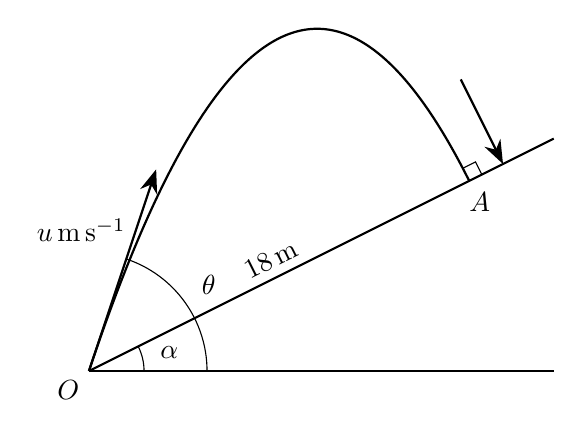
\begin{tikzpicture}[x=0.3cm, y=0.3cm]
\def\OA{18}
\def\tanAlpha{0.5}
\def\tanTheta{3}
\def\planeLen{22}
\def\angleRayLen{6}
\def\velocityArrowLen{9}
\def\impactOffset{1.6}
\def\impactLen{4}
\def\rightAngleSize{0.6}
\def\labelGap{1}
\pgfmathsetmacro{\alph}{atan(\tanAlpha)}
\pgfmathsetmacro{\thet}{atan(\tanTheta)}
\pgfmathsetmacro{\xA}{\OA*cos(\alph)}
\pgfmathsetmacro{\yA}{\OA*sin(\alph)}
\pgfmathsetmacro{\quadCoeff}{(\tanTheta*\xA-\yA)/(\xA*\xA)}

\coordinate (O) at (0,0);
\coordinate (A) at (\xA,\yA);
\coordinate (T) at (\alph:\planeLen);
\coordinate (G) at ({\planeLen*cos(\alph)},0);
\coordinate (H) at (\angleRayLen,0);
\coordinate (P) at (\alph:\angleRayLen);
\coordinate (V) at (\thet:\angleRayLen);
\coordinate (U) at (\thet:\velocityArrowLen);
\coordinate (F) at ($(A)+(\alph:\impactOffset)$);
\coordinate (FTail) at ($(F)+(\alph+90:\impactLen)$);
\coordinate (R1) at ($(A)+(\alph:\rightAngleSize)$);
\coordinate (R2) at ($(R1)+(\alph+90:\rightAngleSize)$);
\coordinate (R3) at ($(A)+(\alph+90:\rightAngleSize)$);

\draw[thick, black] (O) -- (G);
\draw[thick, black] (O) -- (T);
\draw[thick, black, domain=0:\xA, samples=200]
  plot (\x, {\tanTheta*\x - \quadCoeff*\x*\x});

\draw[-{Stealth[length=3mm]}, thick, black] (O) -- (U)
  node[pos=0.7, left] {$u\,\mathrm{m\,s^{-1}}$};
\pic["$\alpha$", draw, angle radius=7mm, angle eccentricity=1.5] {angle=H--O--P};
\pic["$\theta$", draw, angle radius=15mm, angle eccentricity=1.25] {angle=H--O--V};

\draw[-{Stealth[length=3mm]}, thick, black] (FTail) -- (F);
\draw[black] (R1) -- (R2) -- (R3);

\path (O) -- (A) node[midway, above, sloped] {$18\,\mathrm{m}$};

\node[below left] at (O) {$O$};
\node at ($(A)+(\alph-90:\labelGap)$) {$A$};
\end{tikzpicture}
\end{djsSolutionFigure}

Take up the plane and away from the plane as positive. The initial velocity components are \(u\cos(\theta-\alpha)\) and \(u\sin(\theta-\alpha)\), and the corresponding accelerations are \(-g\sin\alpha\) and \(-g\cos\alpha\).

Let \(t>0\) be the time taken to reach \(A\). For each component, the constant acceleration formulae are
\[
s=v_0t+\dfrac12at^2,\qquad v=v_0+at
\]

Here \(v_0\) denotes the initial velocity component. At impact, the velocity component along the plane is zero, so
\begin{align*}
0&=u\cos(\theta-\alpha)-gt\sin\alpha\\
u\cos(\theta-\alpha)&=gt\sin\alpha
\end{align*}

The displacement perpendicular to the plane is zero:
\begin{align*}
0&=ut\sin(\theta-\alpha)-\dfrac12gt^2\cos\alpha\\
u\sin(\theta-\alpha)&=\dfrac12gt\cos\alpha
\end{align*}

Dividing these two component relations and using \(\tan\theta=3\) gives
\begin{align*}
\tan(\theta-\alpha)&=\dfrac{\cos\alpha}{2\sin\alpha}\\
\dfrac{3-\tan\alpha}{1+3\tan\alpha}&=\dfrac{1}{2\tan\alpha}\\
2\tan\alpha(3-\tan\alpha)&=1+3\tan\alpha\\
2\tan^2\alpha-3\tan\alpha+1&=0\\
(2\tan\alpha-1)(\tan\alpha-1)&=0
\end{align*}

Since \(0<\alpha<90^\circ\), the possible angles are
\[
\alpha=\arctan\left(\dfrac12\right)\qquad\text{or}\qquad\alpha=45^\circ
\]

Both satisfy \(\alpha<\theta\), so the particle initially moves away from the plane.

Now apply the displacement formula along the plane, using \(u\cos(\theta-\alpha)=gt\sin\alpha\):
\begin{align*}
18&=ut\cos(\theta-\alpha)-\dfrac12gt^2\sin\alpha\\
&=gt^2\sin\alpha-\dfrac12gt^2\sin\alpha\\
&=\dfrac12gt^2\sin\alpha\\
t^2&=\dfrac{36}{g\sin\alpha}
\end{align*}

Squaring the relation for the initial component along the plane gives
\begin{align*}
u^2\cos^2(\theta-\alpha)&=g^2t^2\sin^2\alpha\\
&=36g\sin\alpha\\
u^2&=\dfrac{36g\sin\alpha}{\cos^2(\theta-\alpha)}
\end{align*}

As \(\tan\theta=3\) and \(\theta\) is acute, \(\cos\theta=\frac{1}{\sqrt{10}}\) and \(\sin\theta=\frac{3}{\sqrt{10}}\), so
\[
\cos(\theta-\alpha)=\cos\theta\cos\alpha+\sin\theta\sin\alpha
=\dfrac{\cos\alpha+3\sin\alpha}{\sqrt{10}}
\]

Substituting the two angles:
\begin{align*}
\alpha=\arctan\left(\dfrac12\right):\quad
u^2&=\dfrac{36g(1/\sqrt5)}{(1/\sqrt2)^2}
=\dfrac{72g}{\sqrt5}\\
\alpha=45^\circ:\quad
u^2&=\dfrac{36g(1/\sqrt2)}{(2/\sqrt5)^2}
=\dfrac{45g}{\sqrt2}
\end{align*}

Using \(g=9.8\,\mathrm{m\,s^{-2}}\), the possible pairs are
\[
(\alpha,u)=(26.6^\circ,\ 17.8\,\mathrm{m\,s^{-1}})
\quad\text{or}\quad
(45.0^\circ,\ 17.7\,\mathrm{m\,s^{-1}})
\qquad\text{(3 s.f.)}
\]

\par\medskip\noindent\textbf{Final answers with \(g = 10\):} \((\alpha,u)=(26.6^\circ,\ 17.9\,\mathrm{m\,s^{-1}})\);\quad \((\alpha,u)=(45.0^\circ,\ 17.8\,\mathrm{m\,s^{-1}})\)
\end{djsSolution}

\newpage

% ---- Question 9 ----
\questionitem
% [Source: _QBT___Solns__Projectile_Motion, Q9]

\begin{figure}[H]
    \centering
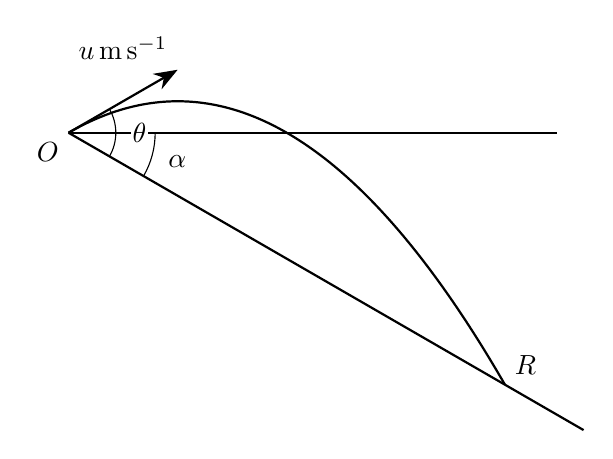
\begin{tikzpicture}[scale=0.32]
\def\incline{30}
\def\launchAngle{60}
\def\speed{10}
\def\grav{10}
\def\planeExtension{1.18}
\def\horizontalExtension{1.12}
\def\velocityLength{5}
\pgfmathsetmacro{\elevation}{\launchAngle-\incline}
\pgfmathsetmacro{\flightTime}{2*\speed*sin(\launchAngle)/(\grav*cos(\incline))}
\pgfmathsetmacro{\xR}{\speed*cos(\elevation)*\flightTime}
\pgfmathsetmacro{\yR}{-\xR*tan(\incline)}
\pgfmathsetmacro{\quadCoeff}{\grav/(2*\speed^2*cos(\elevation)^2)}
\coordinate (O) at (0,0);
\coordinate (R) at (\xR,\yR);
\coordinate (H) at ({\horizontalExtension*\xR},0);
\coordinate (S) at ({\planeExtension*\xR},{\planeExtension*\yR});
\coordinate (V) at (\elevation:\velocityLength);
\draw[thick,black] (O) -- (H);
\draw[thick,black] (O) -- (S);
\draw[thick,black,domain=0:\xR,samples=150] plot (\x,{tan(\elevation)*\x-\quadCoeff*\x^2});
\draw[-{Stealth[length=3mm]},thick,black] (O) -- (V) node[above left] {$u\,\mathrm{m\,s^{-1}}$};
\pic["$\alpha$",draw,angle radius=11mm,angle eccentricity=1.3] {angle=R--O--H};
\pic["$\theta$",draw,angle radius=6mm,angle eccentricity=1.5,pic text options={fill=white,inner sep=0.5pt}] {angle=R--O--V};
\node[below left] at (O) {$O$};
\node[above right] at (R) {$R$};
\end{tikzpicture}
\end{figure}


A small ball $P$ is projected from a point $O$ on a plane which slopes downwards at an angle $\alpha$ to the horizontal, where $0<\alpha<90^\circ$. \\
Its initial speed is $u\,\mathrm{m\,s^{-1}}$, and its initial velocity makes an angle $\theta$ above the downhill direction of the plane. \\
The ball moves in a vertical plane containing a line of greatest slope and next meets the plane at $R$, where $OR=d\,\mathrm{m}$. \\

Assume that air resistance is negligible and that $0<\theta<90^\circ+\alpha$. \\

\begin{enumerate}[label=\textbf{(\alph*)}]
\item Derive an expression for the time of flight in terms of $u$, $\theta$, $\alpha$ and $g$. \\
Hence show that the speed required to reach $R$ satisfies
\[
u^2=\frac{gd\cos^2\alpha}{2\sin\theta\cos(\theta-\alpha)}
\] \marks[-30pt]{8}
\item The point $R$ is fixed. Using a trigonometric identity, determine the minimum possible value of $u$, and the value of $\theta$ for which this minimum occurs. Give your answers in terms of $d$, $g$ and $\alpha$. \marks{4} \\
\item Now take $\alpha=30^\circ$, $d=20$ and $g=10\,\mathrm{m\,s^{-2}}$. The ball is projected with speed $5\sqrt{6}\,\mathrm{m\,s^{-1}}$. Find the two possible values of $\theta$ and the corresponding times of flight, giving the times exactly. \marks{5} \\
\end{enumerate}

\vspace*{10pt}

\begin{djsSolution}
\begin{enumerate}[label=\textbf{(\alph*)}, start=1]
\item
Take horizontal motion to the right and vertical motion upwards as positive. The initial velocity makes an angle \(\theta-\alpha\) with the horizontal, so its components are
\[
v_{x0}=u\cos(\theta-\alpha),\qquad v_{y0}=u\sin(\theta-\alpha)
\]

Let \(t\) be the time of flight. The constant acceleration formula is
\[
s=v_0t+\frac12at^2
\]

With horizontal acceleration zero and vertical acceleration \(-g\), the displacements from \(O\) are
\[
x=u\cos(\theta-\alpha)t,\qquad y=u\sin(\theta-\alpha)t-\frac12gt^2
\]

At \(R\), \(x=d\cos\alpha\) and \(y=-d\sin\alpha\), so \(y=-x\tan\alpha\). Substituting the displacement expressions:
\begin{align*}
-u\cos(\theta-\alpha)t\tan\alpha
&=u\sin(\theta-\alpha)t-\frac12gt^2\\
\frac12gt^2
&=ut\left[\sin(\theta-\alpha)+\cos(\theta-\alpha)\tan\alpha\right]\\
&=\frac{ut}{\cos\alpha}\left[\sin(\theta-\alpha)\cos\alpha+\cos(\theta-\alpha)\sin\alpha\right]\\
&=\frac{ut\sin\theta}{\cos\alpha}
\end{align*}

Since the next meeting with the plane occurs at \(t>0\), dividing by \(t\) gives
\[
t=\frac{2u\sin\theta}{g\cos\alpha}\,\mathrm{s}
\]

Hence, using the horizontal displacement to \(R\):
\begin{align*}
d\cos\alpha
&=u\cos(\theta-\alpha)\left(\frac{2u\sin\theta}{g\cos\alpha}\right)\\
gd\cos^2\alpha
&=2u^2\sin\theta\cos(\theta-\alpha)\\
u^2&=\frac{gd\cos^2\alpha}{2\sin\theta\cos(\theta-\alpha)}
\end{align*}

\item The numerator in part (a) is fixed and positive, so \(u\) is minimised by maximising the denominator. Using the identity \(2\sin A\cos B=\sin(A+B)+\sin(A-B)\):
\[
2\sin\theta\cos(\theta-\alpha)
=\sin(2\theta-\alpha)+\sin\alpha
\leq 1+\sin\alpha
\]

Equality occurs when \(2\theta-\alpha=90^\circ\), giving \(\theta=45^\circ+\frac{\alpha}{2}\), which lies in the permitted interval. Therefore
\begin{align*}
u_{\min}^2
&=\frac{gd\cos^2\alpha}{1+\sin\alpha}\\
&=\frac{gd(1-\sin\alpha)(1+\sin\alpha)}{1+\sin\alpha}\\
&=gd(1-\sin\alpha)
\end{align*}

The minimum speed and its projection angle are
\[
u_{\min}=\sqrt{gd(1-\sin\alpha)}\,\mathrm{m\,s^{-1}},\qquad
\theta=45^\circ+\frac{\alpha}{2}
\]

\item Substituting the given values into the result of part (a):
\begin{align*}
(5\sqrt6)^2
&=\frac{10\times20\cos^2 30^\circ}{2\sin\theta\cos(\theta-30^\circ)}\\
150&=\frac{150}{2\sin\theta\cos(\theta-30^\circ)}\\
2\sin\theta\cos(\theta-30^\circ)&=1\\
\sin(2\theta-30^\circ)+\sin30^\circ&=1\\
\sin(2\theta-30^\circ)&=\frac12
\end{align*}

The permitted interval is \(0<\theta<120^\circ\), so \(-30^\circ<2\theta-30^\circ<210^\circ\). Thus
\begin{align*}
2\theta-30^\circ&=30^\circ\quad\text{or}\quad150^\circ\\
\theta&=30^\circ\quad\text{or}\quad90^\circ
\end{align*}

Using the time of flight from part (a):
\[
t=\frac{2(5\sqrt6)\sin\theta}{10\cos30^\circ}
=2\sqrt2\sin\theta\,\mathrm{s}
\]

The two angles and corresponding times are
\[
\theta=30^\circ:\quad t=\sqrt2\,\mathrm{s},\qquad
\theta=90^\circ:\quad t=2\sqrt2\,\mathrm{s}
\]

\end{enumerate}
\end{djsSolution}

\end{enumerate}
\end{document}
